\CourseSection{Introduction}
\label{sec:introduction}

\CourseSubsection{Motivation and Problem}

Golfers who walk the course must carry their bag or push a cart, and low-handicap golfers rate carrying the bag as the hardest option~\cite{kasper2023golf}. Electric and follow-me carts reduce this effort~\cite{kasper2023golf} but only carry the bag. Golfers must still keep track of every club they take out, and a club left beside a green is easily lost. Club trackers cover part of this problem, but they rely on a phone, can miss shots~\cite{hall2025golfGps}, and do not carry the bag.

\CourseSubsection{Project Objectives}

The \ac{ASCC} is a motorized golf cart that solves both problems at once. It follows the golfer, keeps track of the clubs in the bag, and shows the distance to the green, all without the golfer using a phone. It follows a small \ac{UWB} radio tag carried by the golfer instead of using a camera~\cite{islam2019personFollowing}, so it cannot mistake another person for the golfer. Obstacle sensors and a handheld emergency stop (e-stop) stop the cart when needed.

Each club carries an \ac{RFID} tag, and a reader in the bag, called the smart bag, notices when a club is removed and warns the golfer if the cart moves on without it. The smart bag also blocks the cart from moving toward the golfer while a club is out, since the golfer is about to swing. This is called the club-out interlock.

\CourseSubsection{Project Scope}

The \ac{MVP} covers driving, golfer following, obstacle and emergency stopping, club tracking, and the distance display. Shot tracking, club recommendations, and voice control would add value but are stretch goals, because they depend on the core functions working first. The deliverable is one cart, tested on dry, flat grass with one golfer and one bag. It is not intended for crowded areas, public roads, or rough terrain.

\CourseSubsection{System Overview and Operating Scenario}

Figure~\ref{fig:ascc-system-overview} shows the subsystems and how they interact with the golfer and the course, with a Raspberry Pi coordinating them. The golfer clips on the tag and walks the hole while the cart follows 1 to 3\,m behind. When the golfer stops to hit, the cart stops, and once a club is out it will not move toward the golfer until the club is returned. The display shows the distance to the green and warns if a club is left behind. During testing, a safety operator walks nearby holding the e-stop.

\begin{figure}[htbp]
    \centering
    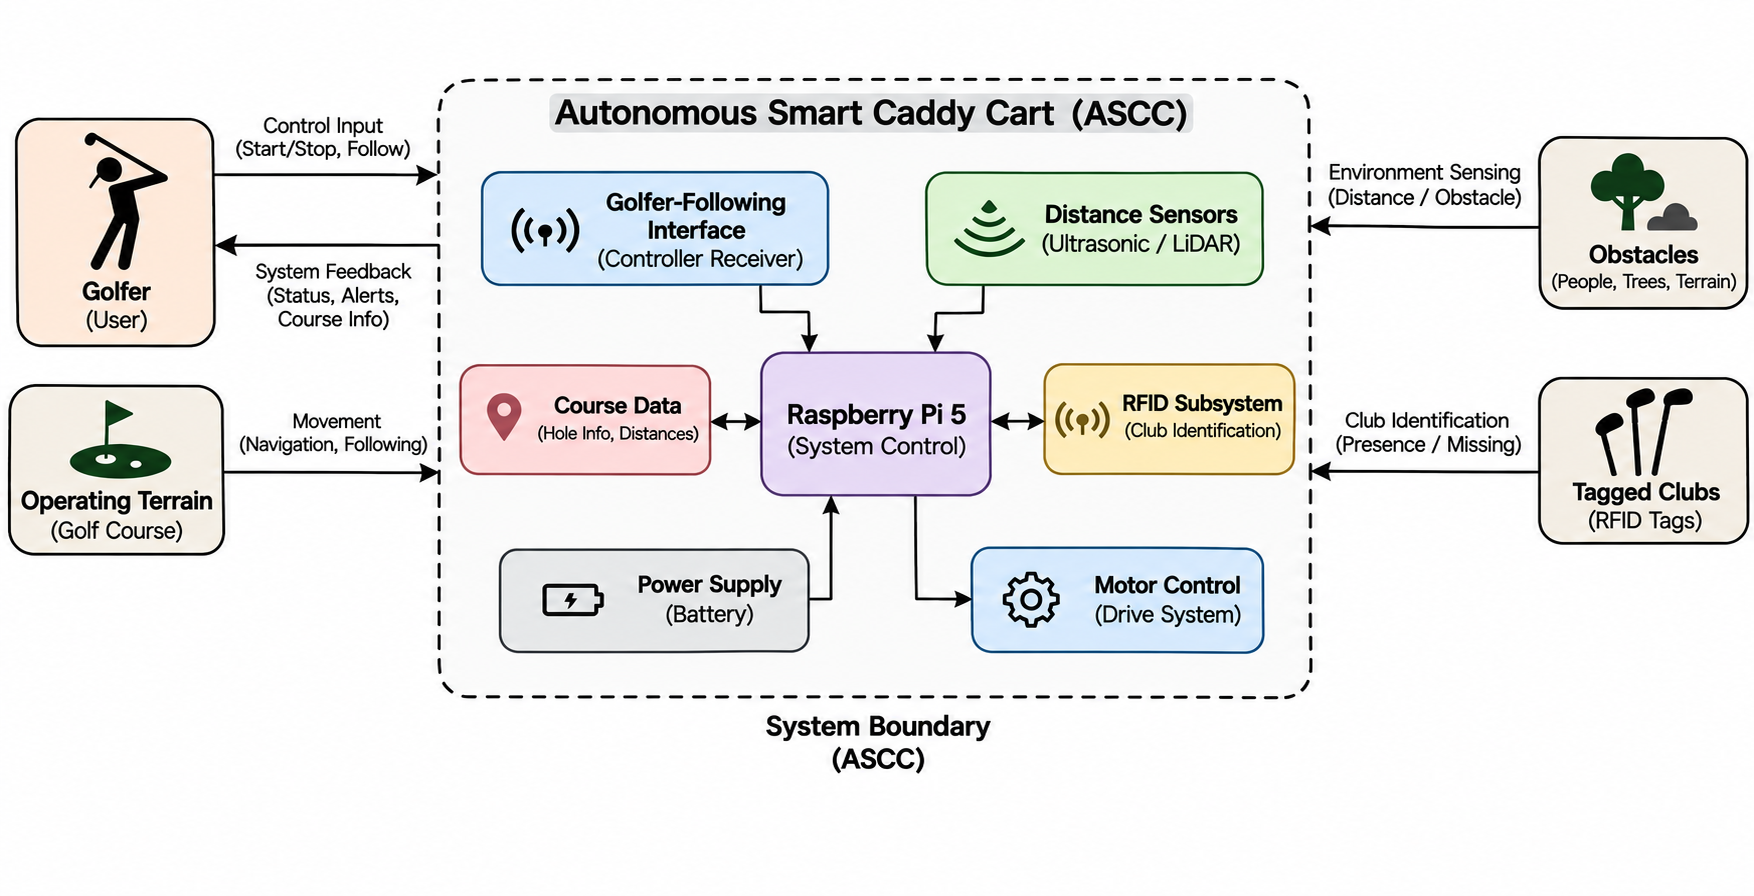
\includegraphics[
        width=0.85\linewidth,
        height=0.2\textheight,
        keepaspectratio
    ]{figures/System Diagram.png}
    \caption{ASCC system overview and external interactions.}
    \label{fig:ascc-system-overview}
\end{figure}

\CourseSubsection{Design Constraints}

The project must stay within the CAD \$600 budget and be finished for the March 2027 demonstration. To save cost, the cart reuses an owned Raspberry Pi, ultrasonic sensors, and golf push cart, and its drive comes from a used hoverboard. Snow in Kingston limits outdoor testing on grass to November and March.
